\documentclass[10pt]{article}
\setlength{\oddsidemargin}{-0.5in} \setlength{\textwidth}{18cm}
\setlength{\topmargin}{-0.7in} \setlength{\textheight}{9.4in}
\usepackage{amssymb}
\usepackage{amsmath,graphicx}
\usepackage{fancyhdr}
%\usepackage[final]{pdfpages} 
\def\R{{\mathbb{ R}}}
\def\N{{\mathbb{ N}}}
\def\C{{\mathbb{ C}}}
\def\Z{{\mathbb{ Z}}}
\def\de{{\bf D\'efinition }}
\def\exe{{\bf Exemples }}


\newcommand{\dis}{\displaystyle}
\newcommand{\vect}{\overrightarrow}
\begin{document}

%------------- En tetes et Pieds de Pages ------------
\pagestyle{fancy}
\renewcommand{\headrulewidth}{0pt}

\fancyhead{}
\fancyhead[L]{
\noindent\noindent\begin{minipage}[c]{2.6cm}

\includegraphics[width=2.5cm]{IMAGES/logo_upsti.png}
\end{minipage}
}

\fancyhead[C]{\rule{12cm}{.5pt}}

\fancyhead[R]{%
\noindent\begin{minipage}[c]{3cm}
\begin{flushright}
\footnotesize{\textit{\textsf{Informatique}}}%
\end{flushright}
\end{minipage}
}

\renewcommand{\footrulewidth}{0.2pt}
\fancyfoot[C]{\footnotesize{\bfseries \thepage}}
\fancyfoot[L]{%
\begin{minipage}[c]{.2\linewidth}
\footnotesize{\textsl{S\'ebastien ROUX}}\\
\footnotesize{\textsl{UPSTI}}
\end{minipage}
\begin{minipage}[c]{.15\linewidth}

\includegraphics[width=2cm]{IMAGES/logoCC.png}
\end{minipage}}


\fancyfoot[R]{\footnotesize{TP Simulation Num\'erique (Euler)}}





\begin{center}
{\Large  \bf TP Euler}\\
\end{center}

\section{Exercice : {\it Asservissement d'un chariot}}

\begin{minipage}[c]{0.6\linewidth}
Consid\'erons le contr\^ole en vitesse du mouvement d'un chariot de technologie analogue \`a ceux situ\'es sur les pistes d'athl\'etisme afin de suivre et filmer les coureurs.

\bigskip

Ce chariot est aliment\'e par une tension \'electrique. La grandeur de sortie est la vitesse de translation.



\end{minipage} \hfill
\begin{minipage}[c]{0.3\linewidth}
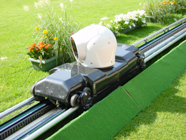
\includegraphics[width=5cm]{IMAGES/camera.jpg}
\end{minipage}





\subsection{En boucle ouverte}
Le comportement temporel  du chariot soumis \`a une tension de commande est mod\'elis\'e par une \'equation diff\'erentielle du premier ordre :

\begin{center}
$\tau_c \frac{d v(t)}{dt} + v(t)= K_c u_c(t)$
\end{center}

L'objectif est d'obtenir la r\'eponse temporelle du syst\`eme \`a une entr\'ee \'echelon (entr\'ee constante) $u_c(t)=U_{mot}$.


\begin{enumerate}
\item \'Ecrire une fonction {\tt{liste\_temps(pas,tmax)}} renvoyant une liste des abscisses en temps \`a partir du {\tt pas} (intervalle entre deux abscisses) et de {\tt tmax} (borne sup\'erieure des temps).

\item \'Ecrire une fonction {\tt ordre1\_euler(K,tau,u,temps)} renvoyant une liste d'ordonn\'ees correspondant \`a la r\'esolution par la m\'ethode d'euler explicite de l'\'equation diff\'erentielle soumise \`a une entr\'ee constante {\tt u} et pour une liste d'abscisses {\tt temps} fournie.

La solution analytique de l'\'equation diff\'erentielle \`a une entr\'ee constante s'\'ecrit : 
\begin{center}
$v(t) = K_c U_{mot}\left(1 - exp\left(-t/\tau_c\right)\right)$
\end{center}

\item \'Ecrire une fonction {\tt ordre1\_th(K,tau,u,temps)} renvoyant une liste d'ordonn\'ees correspondant \`a la solution analytique pr\'ec\'edente pour une liste d'abscisses {\tt temps} fournie.

Nous allons t\^acher de superposer le trac\'e de la r\'eponse analytique avec les trac\'es approch\'es par la m\'ethode d'Euler pour diff\'erentes valeurs de pas.

Les valeurs num\'eriques des param\`etres sont :
$K_c=0.5 m.s^{-1}.V^{-1}$, $\tau_c = 1 s$, $U_{mot} = 5 V$ et $t_{max}=5 s$


\item Tester ces lignes afin de prendre en main les fonctionnalit\'es de trac\'es 
\begin{verbatim}
#Importation des modules
import matplotlib.pyplot as plt #module de gestion des traces
##########################################

Les fonctions etant definies

##########################################
#Les elements de base
##########################################
x=liste_temps(tmax,0.1)          #une liste d'abscisse
z=ordre1_th(K_c,tau_c,U_mot,x) #une liste d'ordonnee de meme taille que celle des abscisses
plt.plot(x,z,'-')  #Stocke en memoire le trace avec ses options
plt.show()  #pour afficher les traces en memoire

###############################
#Pour enrichir le trace
###############################
marqueurs = ['^', '+', '.', 'x', '*', 'o'] #Les marqueurs
couleurs = ['b', 'g', 'r', 'c', 'm', 'y', 'k', 'w'] #Les couleurs
style = ['-', '--', '-.', ':'] #Les styles de trait

plt.plot(x,z,'--',marker='^',color='r',linewidth=2,label='analytique')  
plt.title('Reponse temporelle') #titre du trace
plt.legend(loc='lower right') #positionne les \'etiquettes
plt.xlabel('temps') #legende de l'axe des abscisses
plt.ylabel('vitesse') #legende de l'axe des ordonnees
plt.show()  #pour afficher les traces en memoire
\end{verbatim}

\item Tracer sur un m\^eme graphe la solution analytique ainsi que la solution approch\'ee par la m\'ethode d'Euler pour des pas de [0.3,0.5,0.7,1].

\end{enumerate}


\subsection{En boucle ferm\'ee}
Afin de contr\^oler le chariot, le pilotage s'effectue en boucle ferm\'ee. Une consigne de vitesse $V_{cons}(t)$ est impos\'ee. Cette consigne est compar\'ee \`a la vitesse du chariot $v(t)$. L'\'ecart g\'en\'er\'ee est adapt\'ee par un gain r\'eglable $K_A$, soit $u_c(t)=K_A\epsilon(t)$.


\begin{figure}[!hbt]
\begin{center}
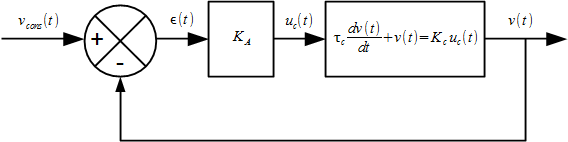
\includegraphics[width=12cm]{IMAGES/BF.png}
\end{center}
\end{figure}


\begin{enumerate}
\item \'Ecrire une fonction {\tt ordre1\_BF(ka,k,tau,vc,temps)} renvoyant une liste d'ordonn\'ees correspondant \`a la r\'esolution par la m\'ethode d'Euler explicite du syst\`eme en boucle ferm\'ee
\item Tracer la r\'eponse du syst\`eme pour une vitesse de consigne constante $V_c=6m.s^{-1}$ et un gain d'adaptation $K_A=20 V.s.m^{-1}$
\end{enumerate}


\subsection{Avec prise en compte de la saturation}

Le choix d'un gain $K_A$ \'elev\'e permet de gagner en pr\'ecision et rapidit\'e. Toutefois, la tension d'alimentation du chariot est \'ecr\^et\'ee \`a +12V ou -12V. Il faut donc en tenir compte dans notre mod\'elisation.

\begin{figure}[!hbt]
\begin{center}
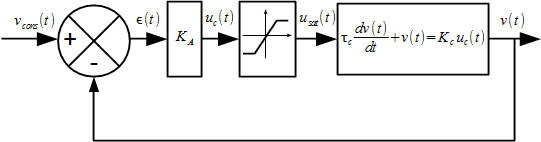
\includegraphics[width=12cm]{IMAGES/BF_sat.png}
\end{center}
\end{figure}

\begin{enumerate}
\item \'Ecrire une fonction {\tt ordre1\_BFsat(ka,k,tau,vc,umax,temps)} correspondant \`a la r\'esolution par la m\'ethode d'Euler explicite du syst\`eme en boucle ferm\'ee avec prise en compte de la saturation. La vitesse du chariot ainsi que la tension d'alimentation du chariot seront r\'ecup\'er\'ees en sortie.
\item  Tracer les r\'eponses superpos\'ees avec et sans saturation, ainsi que la tension d'alimentation du chariot pour une vitesse de consigne constante $V_c=6m.s^{-1}$ et un gain d'adaptation $K_A=20 V.s.m^{-1}$
\end{enumerate}



\section{Exercice : {\it Utilisation des m\'ethodes Python}}
Il est possible d'utiliser des modules Python pour int\'egrer des \'equations diff\'erentielles. \\
Voir : {\tt http://docs.scipy.org/doc/scipy/reference/tutorial/integrate.html}\\
On donne ici un exemple avec l'\'equation diff\'erentielle $y'(t)=2y(t)-(t+1)\sqrt{y(t)}$ de solution g\'en\'erale $y(t)=(\frac12 t+Ce^{-t})^2.$\\ On commence par importer les modules n\'ecessaires. 
On cr\'ee les abscisses dans le tableau $x$, dans le tableau $y$ on met la solution donn\'ee par {\tt integrate.odeint} de param\`etres la fonction $f$ telle que $y'=f(y,t)$, la condition initiale $y_0$ et la liste des abscisses.\\
Pour comparer, on a mis la vraie solution dans la liste $yvraie$ et on a trac\'e les deux graphes.
\begin{verbatim}
import scipy.integrate
import math
import matplotlib.pyplot as plt
def f(y,t):
    return(-2*y+(t+1)*math.sqrt(y))

n=50
a=0
b=5
x=[a+k*(b-a)/n for k in range(n)]
y=scipy.integrate.odeint(f,1,x)
yvraie=[(0.5*t+math.exp(-t))**2 for t in x]

plt.plot(x,y,'*',color='red')
plt.plot(x,yvraie)
plt.show()
\end{verbatim}

Reprendre ce code pour r\'esoudre 
$y'(t)+e^{t-y(t)}=0.$ La solution g\'en\'erale est $y(t)=\ln(C-e^t)$ pour tout $t$ tel que $C-e^t>0.$ On va prendre $C=4,a=0,b=1$ et on essaiera pour plusieurs valeurs de $n.$

\section{Exercice : {\it R\'esolution d'une \'equation diff\'erentielle du second degr\'e}}

Consid\'erons l'\'equation diff\'erentielle \`a coefficients constants du second ordre suivante:

\begin{center}
$\frac{1}{{\omega_0}^2} \frac{d^2 x(t)}{dt^2} + \frac{2 \xi}{\omega_0} \frac{dx(t)}{dt} + x(t)=K u(t)$
\end{center}


Ce type de mod\'elisation est largement rencontr\'e que ce soit en \'electrocin\'etique sur un circuit RLC par exemple o\`u en m\'ecanique \`a l'issue de l'application des lois de Newton.

L'objectif va \^etre de tracer la r\'eponse temporelle \`a une entr\'ee constante $u(t)=U_0$ en utilisant la m\'ethode d'Euler.


En fait, il s'agit de construire un syst\`eme de deux \'equations coupl\'ees :


$\left\lbrace 
\begin{array}{lcl} 
\frac{dx(t)}{dt}=v(t)\\ 
\frac{1}{{\omega_0}^2} \frac{d v(t)}{dt} + \frac{2 \xi}{\omega_0} v(t) + x(t)=K u(t) 
\end{array}\right.$


Soit :

$\left\lbrace 
\begin{array}{lcl} 
\frac{dx(t)}{dt}=f1(v,x,t)\\
\frac{dv(t)}{dt}=f2(v,x,t)
\end{array}\right.$

Les conditions initiales sont alors le couple vitesse, position $(v_0,x_0)$.

\begin{enumerate}
\item Pr\'eciser les expressions des fonctions $f1(v,x,t)$ et $f2(v,x,t)$.

\item \'Ecrire une fonction {\tt ordre2\_euler(K,w0,xi,u0,v0,x0,temps)} renvoyant une liste d'ordonn\'ees pour la position et une autre pour la vitesse \`a partir d'une liste d'abscisses {\tt temps} fournie.

On pose $K=10$, $U_0=5V$, $\omega_0=5 rad/s$, 

\item Proposer une suite d'instructions afin de tracer la r\'eponse de cette \'equation diff\'erentielle avec des conditions initiales nulles et pour des valeurs de facteur d'amortissement ($\xi=\frac{1}{2Q}$ avec $Q$ le facteur de qualit\'e) $xi=[0.3,0.69,1,2,5]$

Nous allons essayer d'utiliser la m\'ethode de r\'esolution implant\'ee dans Python et mis en \'evidence pr\'ec\'edemment ({\tt integrate.odeint}).

Cette m\'ethode n\'ecessite de pr\'esenter l'\'equation sous la forme :$\frac{dz}{dt}=f(z,t)$

Pour y arriver, nous allons consid\'erer que Z est un tuple constitu\'e des variables  $\frac{dx(t)}{dt}=v(t)$ la vitesse et $x$ la position. Soit $z=(\frac{dx(t)}{dt},x(t))=(v(t),x(t))$

Les conditions initiales sont alors $z_0=(v_0,x_0)$

\item Tester les lignes suivantes correspondant \`a la r\'esolution de l'\'equation diff\'erentielle d'ordre 2 pour un $\xi=0.3$
\begin{verbatim}

###################################
###Resolution avec les methodes Python

import scipy.integrate
import math
import matplotlib.pyplot as plt
import numpy

def f(z,t):
    v,p=z
    return((K*u-p-2*xi*v/w_0)*((w_0)**2),v)


K=1
w_0=5
xi=0.3
u=5
   
x=liste_temps(10,0.01)       #Liste abscisses
z0 = [0,0]                    #conditions initiales
z = scipy.integrate.odeint (f, z0, x) #resolution python

y=z[:,1] #Pour avoir la deuxieme colonne (position, environnement numpy)


plt.plot(x,y,'--',color='r',marker='+')
plt.show()  

\end{verbatim} 

\end{enumerate}



\newpage
\begin{verbatim}
#############################################
#####Asservissement d'un chariot
#Importation des modules
import matplotlib.pyplot as plt
import math


#Definition des parametres
K_c=0.5
tau_c=1
U_mot=5
pas = 0.5
tmax=6

#Definition d'une fonction abscisse des temps
def liste_temps(tmax,pas):
    '''Renvoie une liste des abscisses en temps 
    a partir du pas et de la borne superieure des temps'''
    t=0
    temps=[0]
    while t<=(tmax-pas):
        t=t+pas
        temps=temps+[t]
    return (temps)
    
#Definition d'une fonction premier ordre 
def ordre1_euler(k,tau,u,temps):
    ''' Renvoie une liste des ordonnees pour un premier ordre
    soumis a un echelon u de tension 
    pour une liste abscisse des temps fournie'''
    s=0
    sortie=[0]
    for i in range(1,len(temps)):
        f=(k*u-s)/tau
        s=s+f*(temps[i]-temps[i-1])
        sortie=sortie + [s]
    return sortie
    
#reponse analytique d'un premier ordre
def ordre1_th(k,tau,u,temps):
    s=[0]*(len(temps))
    for i in range(len(temps)):
        s[i]=k*u*(1-math.exp(-temps[i]/tau))
    return s
  


#Les traces 

#Trace reponse theorique    
x=liste_temps(tmax,0.1)
z=ordre1_th(K_c,tau_c,U_mot,x)
plt.plot(x,z,'-')


#Trace superpose pour differents pas de temps
marqueurs = ['^', '+', '.', 'x', '*', 'o'] #Les marqueurs
couleurs = ['b', 'g', 'r', 'c', 'm', 'y', 'k', 'w'] #Les couleurs
style = ['-', '--', '-.', ':']
k=0
for i in (0.3,0.5,0.7,1):
    x=liste_temps(tmax,i)
    y=ordre1_euler(K_c,tau_c,U_mot,x)
    plt.plot(x,y,'--',color=couleurs[k],marker=marqueurs[k])
    k=k+1


#Affichage superpose des courbes
plt.show()
  


#Reponse en boucle fermee

#Premier ordre en boucle fermee sans prise en compte de la saturation
def ordre1_BF(ka,k,tau,vc,temps):
    ''' Renvoie une liste des ordonnees pour un premier ordre
    soumis a un echelon u de tension 
    pour une liste abscisse des temps fournie'''
    s=0
    sortie=[0]
    for i in range(1,len(temps)):
        u=ka*(vc-s)
        f=(k*u-s)/tau
        s=s+f*(temps[i]-temps[i-1])
        sortie=sortie + [s]
    return sortie

#Premier ordre en boucle fermee avec prise en compte de la saturation
def ordre1_BFsat(ka,k,tau,vc,umax,temps):
    ''' Renvoie une liste des ordonnees pour un premier ordre
    soumis a un echelon u de tension 
    pour une liste abscisse des temps fournie'''
    s=0
    sortie=[0]
    tension=[0]
    for i in range(1,len(temps)):
        u=ka*(vc-s)
        if u>umax:
            u=umax
        elif u<-umax:
            u=-umax
        f=(k*u-s)/tau
        s=s+f*(temps[i]-temps[i-1])
        sortie=sortie + [s]
        tension = tension +[u]
    return sortie, tension

#Les traces 
#trace superpose pour differents pas de temps   

x=liste_temps(5,0.001)
y=ordre1_BF(20,K_c,tau_c,6,x)
z , us =ordre1_BFsat(20,K_c,tau_c,6,12,x)
plt.plot(x,y,'--')
plt.plot(x,z,'--')
plt.plot(x,us,'--')
plt.show()  



###################################
###Resolution avec les methodes Python

import scipy.integrate
import math
import matplotlib.pyplot as plt

def f(y,t):
    return(-math.exp(t-y))

n=50
a=0
b=1
C=4

x=[a+k*(b-a)/n for k in range(n)]

y=scipy.integrate.odeint(f,math.log(C-1),x)
yvraie=[math.log(C-math.exp(t)) for t in x]

plt.plot(x,y,'*',color='red')
plt.plot(x,yvraie)
plt.show()


#################################################
#R�solution d'une �quation diff�rentielle d'ordre 2

#Importation des modules
import matplotlib.pyplot as plt
import math


#D�finition des param�tres
K=10
w_0=5
U_mot=5
pas = 0.5
tmax=5


    
#D�finition d'une fonction deuxi�me ordre
#Equation du type 
def ordre2_euler(w_0,xi,K,u,temps):
    ''' Renvoie une liste des ordonn�es pour un premier ordre
    soumis � un �chelon u de tension 
    pour une liste abscisse des temps fournie'''
    p=0
    v=0
    position=[0]
    vitesse=[0]
    for i in range(1,len(temps)):
        f1=(K*u-p-2*xi*v/w_0)*((w_0)**2)
        f2=v
        v2=v+f1*(temps[i]-temps[i-1])
        p2=p+f2*(temps[i]-temps[i-1])
        position=position + [p2]
        vitesse=vitesse+[v2]
        v=v2
        p=p2
    return position, vitesse
    
#Les trac�s 

#Trac� reponse    
x=liste_temps(10,0.01)

#Trac� superpos� pour diff�rents pas de temps
marqueurs = ['^', '+', '.', 'x', '*', 'o'] #Les marqueurs
couleurs = ['b', 'g', 'r', 'c', 'm', 'y', 'k', 'w'] #Les couleurs
style = ['-', '--', '-.', ':']
k=0
#Pour diff�rentes valeurs de xi
for i in (0.3,0.69,1,2,5):
    y,z=ordre2_euler(w_0,i,K,U_mot,x)
    plt.plot(x,y,'--',color=couleurs[k],marker=marqueurs[k])
    k=k+1


#Affichage superpose des courbes
plt.show()


###########################################
###Resolution avec les methodes Python
#Utilisation de integrate.odeint

import scipy.integrate
import numpy

def f(z,t):
    v,p=z
    return((K*u-p-2*xi*v/w_0)*((w_0)**2),v)


xi=0.3
   
x=liste_temps(10,0.01)
z0 = [0,0]
z = scipy.integrate.odeint (f, z0, x)

y=z[:,1] #Pour avoir la deuxi�me colonne (position, environnement numpy)
plt.plot(x,y,'--',color='r',marker='+')
plt.show()
  

\end{verbatim}
\end{document}
